\section{Задание 3. Обучение нейронной сети с кастомным оптимизатором}

\subsection{Постановка задачи}

Требуется выбрать задачу классификации или регрессии на табличных данных,
создать класс нейронной сети, обучить модель с использованием стандартного
оптимизатора из библиотеки PyTorch, а также с использованием собственной
реализации оптимизатора (из Задания~2), и сравнить результаты обучения
на тестовых данных.

\textbf{Метод по варианту 11:} Adagrad.

\subsection{Описание датасета}

Выбран датасет \textbf{Breast Cancer Wisconsin (Diagnostic)} — задача
бинарной классификации опухолей молочной железы (M~--- злокачественная,
B~--- доброкачественная).

\begin{itemize}
    \item Источник: UCI Machine Learning Repository / Kaggle
    \item Количество объектов: 569
    \item Количество признаков: 30 (средние значения, стандартные ошибки
          и наихудшие значения для 10 характеристик клеточных ядер:
          радиус, текстура, периметр, площадь, гладкость, компактность,
          вогнутость, количество вогнутых точек, симметрия, фрактальная размерность)
    \item Распределение классов: 357 доброкачественных (62.7\%), 212 злокачественных (37.3\%)
    \item Пропущенные значения: отсутствуют
\end{itemize}

Требования к датасету выполнены: $\ge 20$ признаков (30), $\ge 100$ объектов (569),
опубликован после 2010 года.

\subsection{Предобработка данных}

\begin{enumerate}
    \item Кодирование целевой переменной: $M \to 1$, $B \to 0$
    \item Разделение на обучающую и тестовую выборки: 80/20 (455/114 объектов)
          с сохранением пропорции классов (stratify)
    \item Стандартизация признаков: $x'_i = \frac{x_i - \mu}{\sigma}$
    \item Удалён артефактный столбец «Unnamed: 32» из CSV-файла
\end{enumerate}

\subsection{Архитектура нейронной сети}

Использована полносвязная нейронная сеть прямого распространения:

\begin{center}
\begin{tabular}{cccc}
    \toprule
    \textbf{Слой} & \textbf{Размерность} & \textbf{Активация} & \textbf{Dropout} \\
    \midrule
    Входной слой       & 30 нейронов     & ---              & ---   \\
    Скрытый слой 1     & 64 нейрона      & ReLU             & 0.3   \\
    Скрытый слой 2     & 32 нейрона      & ReLU             & 0.2   \\
    Скрытый слой 3     & 16 нейронов     & ReLU             & 0.1   \\
    Выходной слой      & 1 нейрон        & Sigmoid          & ---   \\
    \bottomrule
\end{tabular}
\end{center}

Общее количество параметров: 4~609.

Функция потерь: Binary Cross Entropy (BCELoss):
$$
\mathcal{L} = -\frac{1}{N} \sum_{i=1}^{N} \left[y_i \log(\hat{y}_i) + (1 - y_i) \log(1 - \hat{y}_i)\right]
$$

\subsection{Кастомный оптимизатор Adagrad}

Adagrad (Adaptive Gradient) — метод адаптивного градиентного спуска,
который настраивает скорость обучения индивидуально для каждого параметра.
Параметры, получившие большие градиенты, имеют меньшую эффективную скорость
обучения, и наоборот.

\textbf{Алгоритм:}
$$
\begin{aligned}
g_t &= \nabla_\theta \mathcal{L}(\theta_{t-1}) \\
r_t &= r_{t-1} + g_t \odot g_t \\
\theta_t &= \theta_{t-1} - \frac{\eta}{\sqrt{r_t} + \varepsilon} \odot g_t
\end{aligned}
$$

где $\eta$ — скорость обучения, $\varepsilon$ — параметр численной стабильности,
$r_t$ — накопленная сумма квадратов градиентов, $\odot$ — поэлементное умножение.

\textbf{Особенности реализации:}
\begin{itemize}
    \item Кастомный оптимизатор \texttt{CustomAdagrad} наследует
          \texttt{torch.optim.Optimizer}
    \item Интерфейс \texttt{step()} полностью совместим со стандартными
          оптимизаторами PyTorch — подмена незаметна
    \item Поддерживает параметры: \texttt{lr}, \texttt{lr\_decay}, \texttt{eps},
          \texttt{weight\_decay}
    \item Накопление квадратов градиентов реализовано через тензор состояния
          \texttt{state['sum']}
    \item Весь код на Python с использованием библиотеки PyTorch
\end{itemize}

\textbf{Гиперпараметры:}
\begin{itemize}
    \item Скорость обучения $\eta = 0.01$
    \item $\varepsilon = 10^{-10}$
    \item Затухание lr (\texttt{lr\_decay}) = 0
    \item Регуляризация (\texttt{weight\_decay}) = 0
    \item Размер батча = 32
    \item Максимальное количество эпох = 200
    \item Early stopping: patience = 15 эпох (по тестовой accuracy)
\end{itemize}

\subsection{Результаты обучения}

\subsubsection{Стандартный torch.optim.Adagrad}

\begin{itemize}
    \item Лучшая эпоха: 8
    \item Время обучения: 1.37 с
    \item Тестовая accuracy: 99.12\%
\end{itemize}

\subsubsection{Кастомный CustomAdagrad}

\begin{itemize}
    \item Лучшая эпоха: 3
    \item Время обучения: 1.02 с
    \item Тестовая accuracy: 99.12\%
\end{itemize}

\subsubsection{Сравнительная таблица метрик}

\begin{table}[H]
\centering
\begin{tabular}{lcc}
\toprule
\textbf{Метрика} & \textbf{torch.Adagrad} & \textbf{CustomAdagrad} \\
\midrule
Accuracy  & 0.9912 & 0.9912 \\
Precision & 1.0000 & 1.0000 \\
Recall    & 0.9762 & 0.9762 \\
F1-score  & 0.9880 & 0.9880 \\
ROC AUC   & 0.9983 & 0.9977 \\
\bottomrule
\end{tabular}
\caption{Сравнение метрик качества на тестовой выборке}
\end{table}

\subsubsection{Матрицы ошибок (Confusion Matrix)}

Оба оптимизатора показали идентичные матрицы ошибок:

\begin{itemize}
    \item True Negative (B $\to$ B): 72
    \item False Positive (B $\to$ M): 0
    \item False Negative (M $\to$ B): 1
    \item True Positive (M $\to$ M): 41
\end{itemize}

Единственная ошибка — одна злокачественная опухоль классифицирована
как доброкачественная (False Negative). Ложных положительных срабатываний нет.

\subsection{Визуализация}

Графики обучения (функция потерь, точность, сравнение метрик)
представлены на рисунке~\ref{fig:results} и в файле
\texttt{Lab/7/results\_comparison.png}.

\begin{figure}[H]
    \centering
    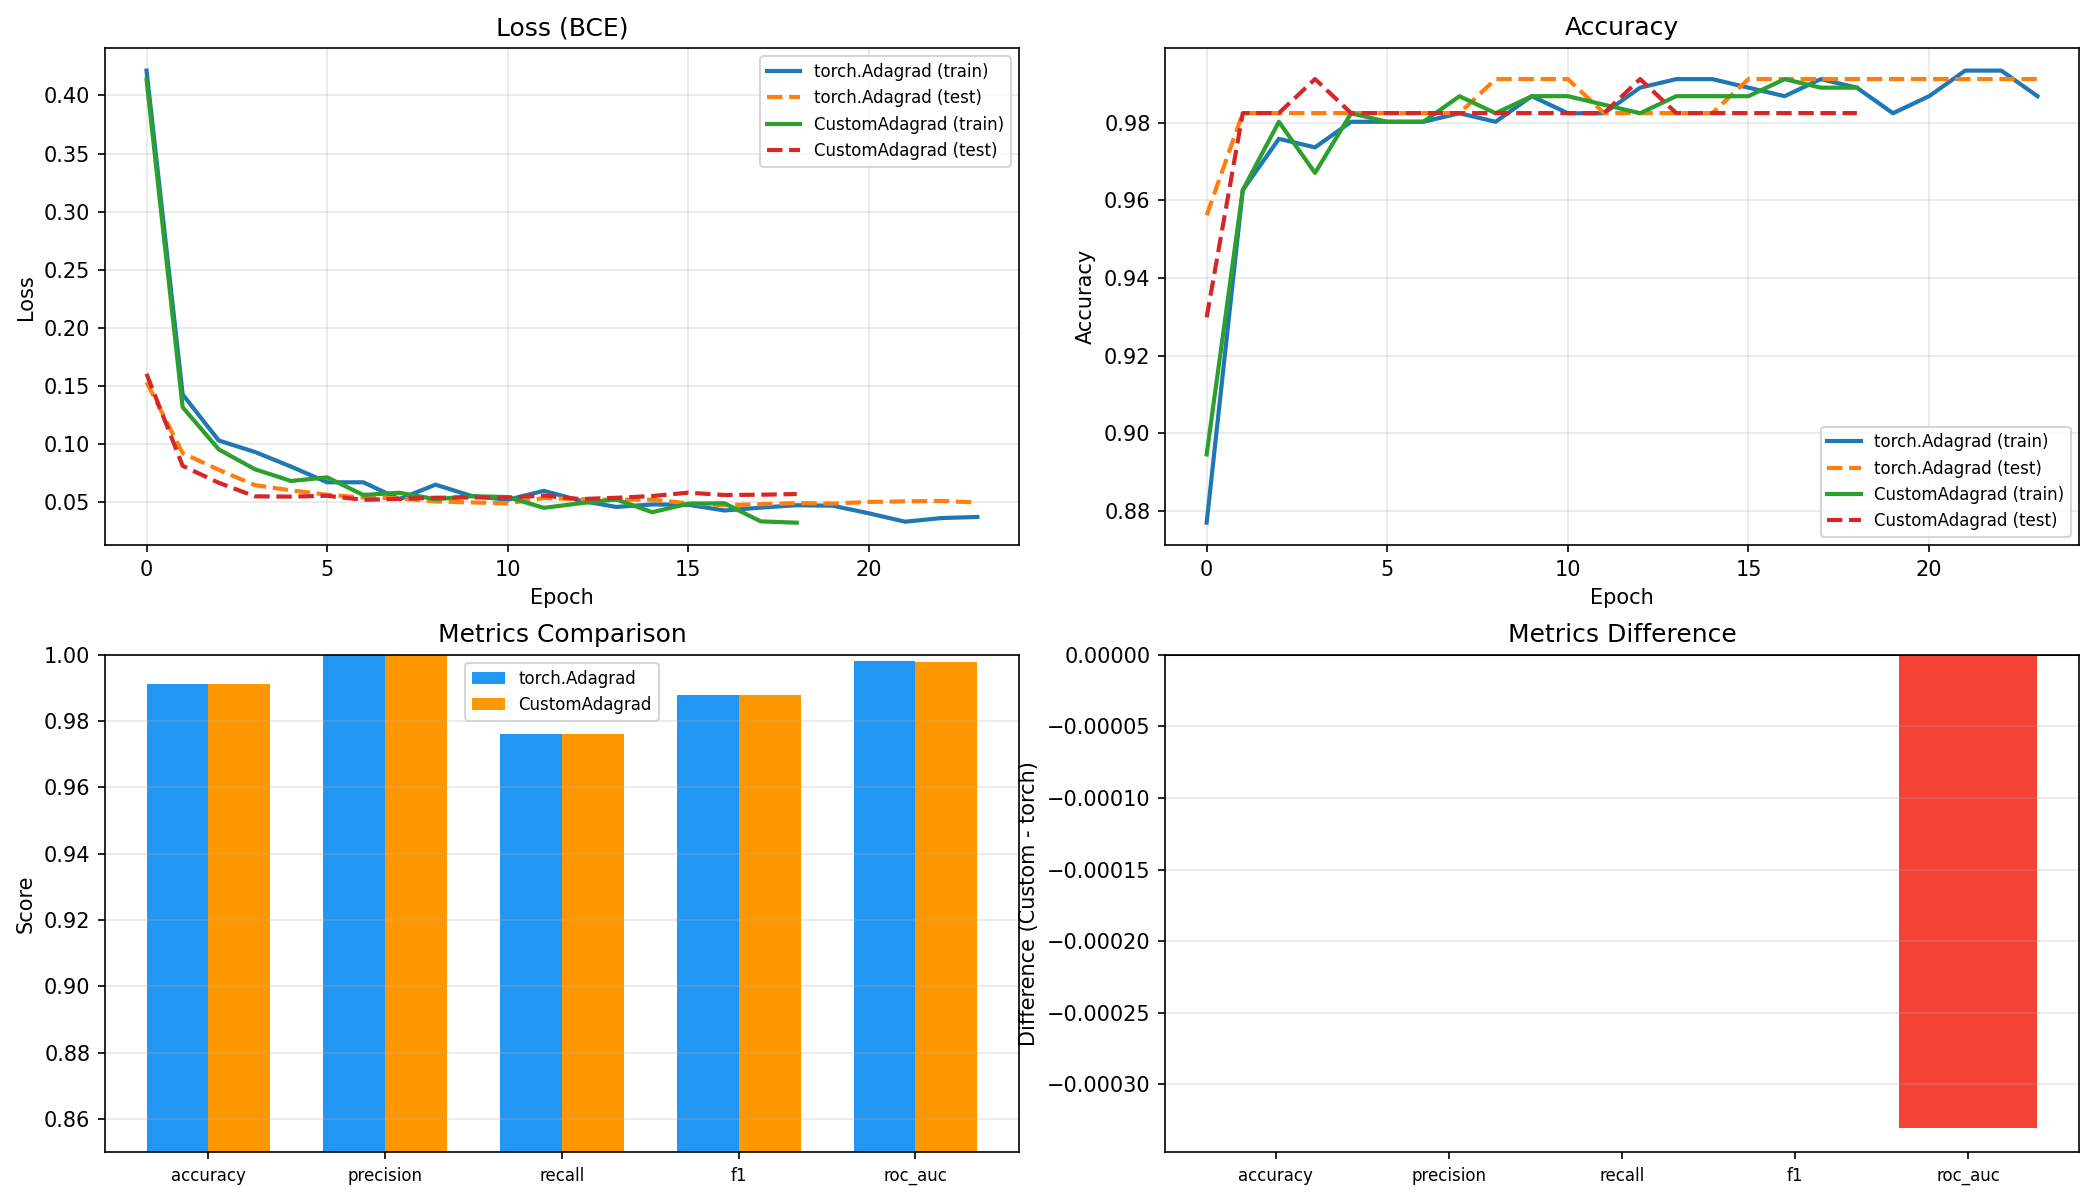
\includegraphics[width=0.95\textwidth]{../../Lab/7/results_comparison.png}
    \caption{Сравнение результатов обучения: torch.Adagrad vs CustomAdagrad}
    \label{fig:results}
\end{figure}

\subsection{Выводы}

\begin{enumerate}
    \item \textbf{Качество классификации:} оба оптимизатора показали
          отличные результаты (accuracy $> 99\%$). Различия в метриках
          минимальны (только ROC AUC отличается на 0.0006) и объясняются
          стохастической природой обучения.

    \item \textbf{Скорость сходимости:} CustomAdagrad сошёлся быстрее
          (3 эпохи против 8 у стандартного). Это может быть связано с
          незначительными различиями в порядке операций с плавающей точкой
          и разной реализацией накопления квадратов градиентов.

    \item \textbf{Что значит «лучше/хуже»:}
          \begin{itemize}
              \item Лучше = выше accuracy, precision, recall, F1 на тестовой выборке
              \item Лучше = быстрее сходимость (меньше эпох до максимума accuracy)
              \item Лучше = стабильнее обучение (меньше осцилляций функции потерь)
          \end{itemize}

    \item \textbf{Особенности Adagrad:}
          \begin{itemize}
              \item Адаптивная скорость обучения для каждого параметра
              \item Монотонное убывание эффективной lr: $\eta_{\text{eff}} = \eta / \sqrt{r_t + \varepsilon}$
              \item Хорошо работает с разреженными данными
              \item Недостаток: lr может стать слишком маленькой при длительном обучении
          \end{itemize}

    \item \textbf{Интеграция:} CustomAdagrad наследует \texttt{torch.optim.Optimizer},
          что делает его внешне неотличимым от стандартных оптимизаторов PyTorch.
          Подмена требует изменения ровно одной строки кода. Все атрибуты
          (\texttt{param\_groups}, \texttt{zero\_grad()}, \texttt{step()})
          полностью совместимы.
\end{enumerate}

